\documentclass{gescons}

\genre {Resumo do Biênio}
\author{Por Luziânia Medeiros e Paulo Abrantes}
\title{Conscienciologia em Expansão: Distribuição de Publicações no Japão e Europa}

\begin{document}
    \makeentrevistatitle
    %\maketitle

    %\fullwidthimage{fields}{b}

    %\coverart{back/editorial}
    \coverart{../fundo-generico.png}
    
%    \begin{multicols}{2}

%\begin{center}
%    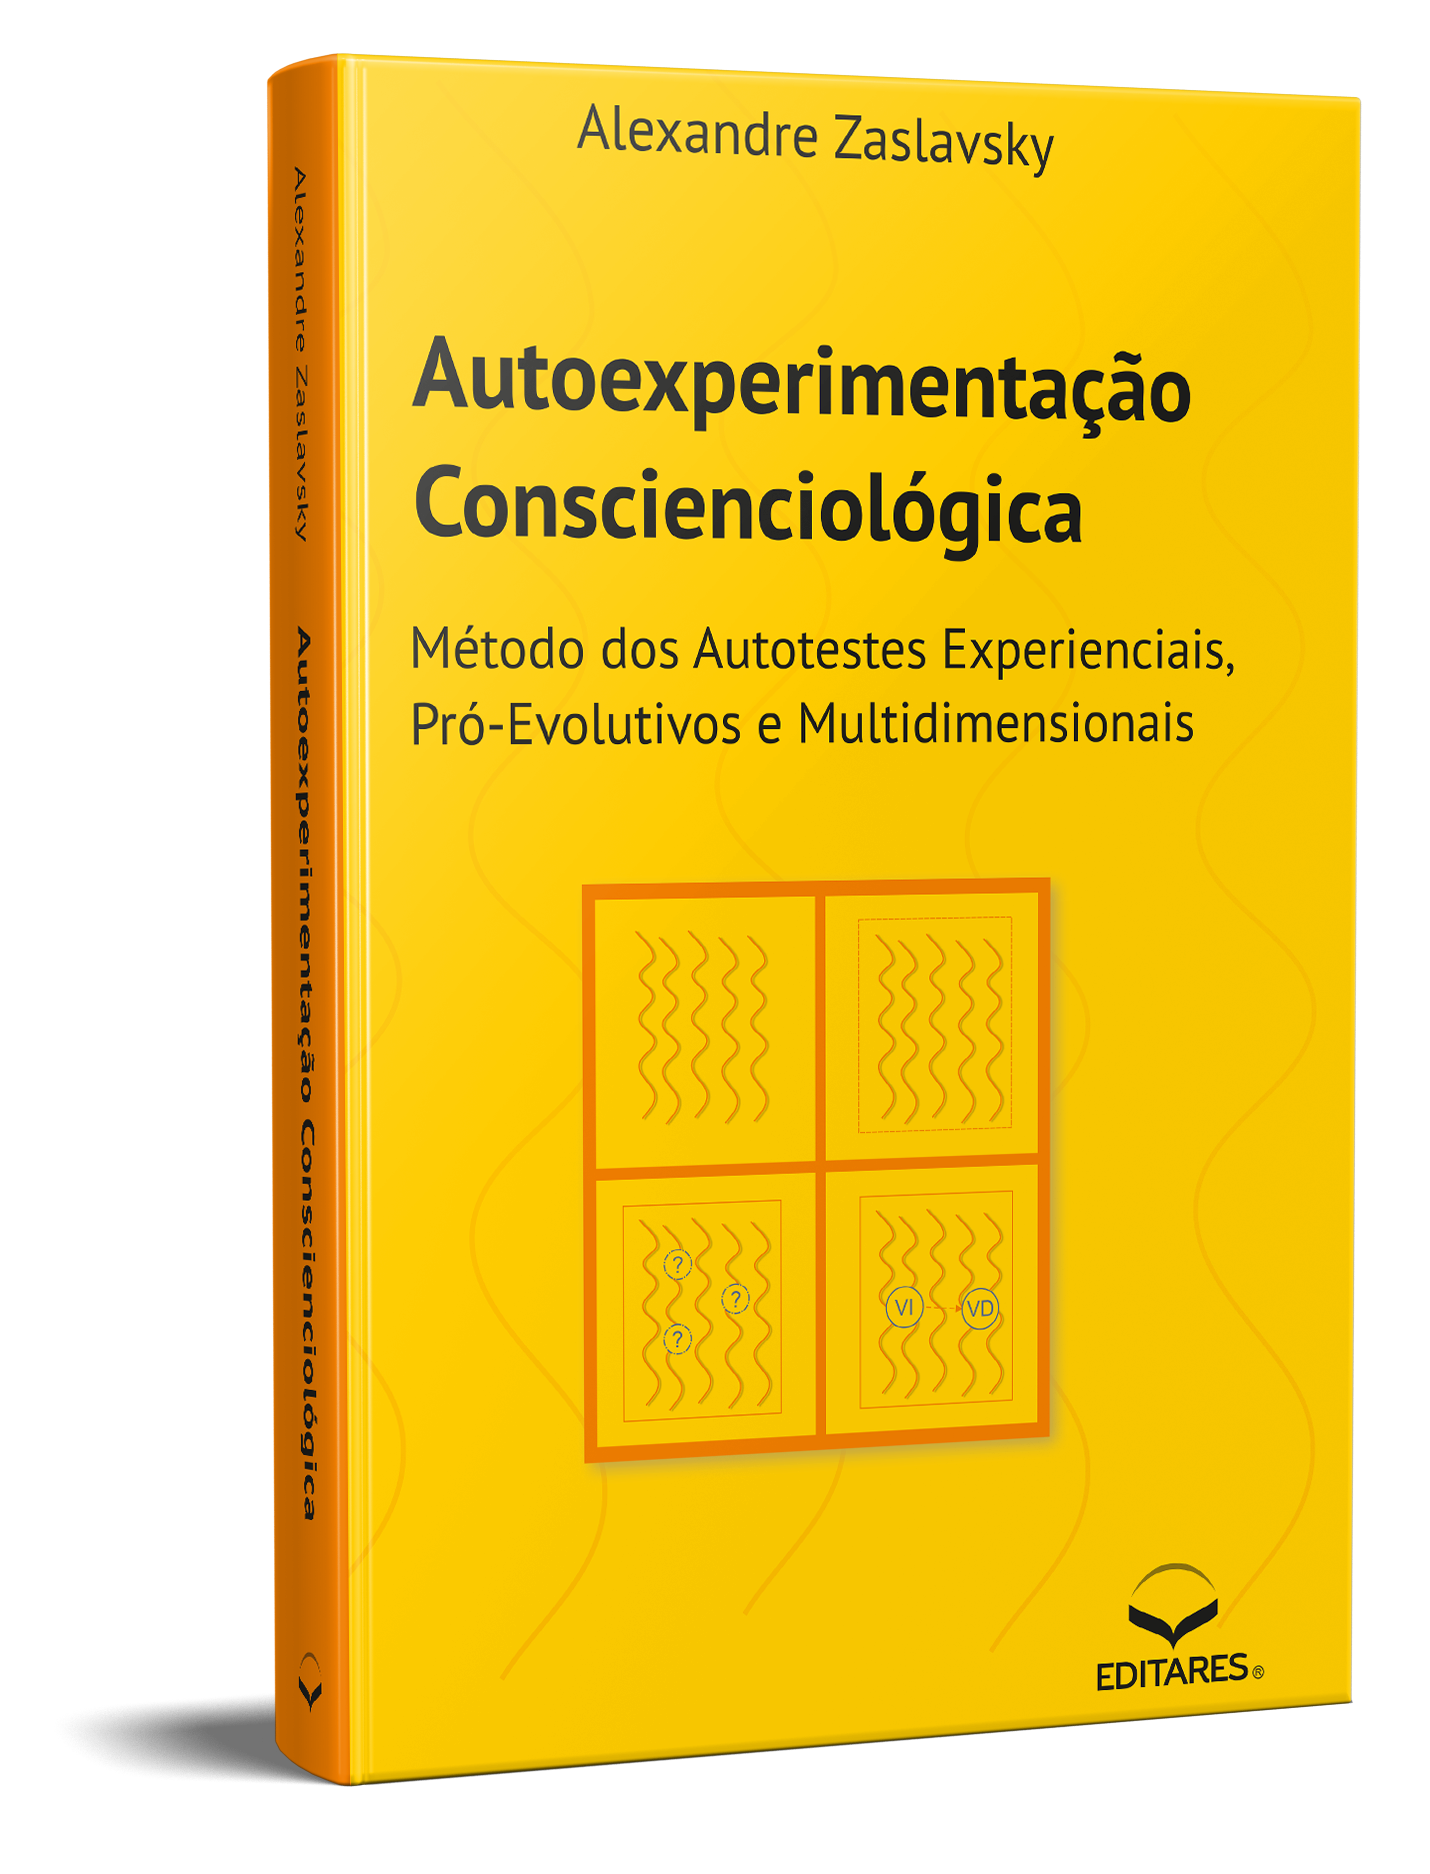
\includegraphics[width=4cm]{articles/entrevista/mockups/Alexandre-Zas.png}
%\end{center}


% \subsection*{Coordenadores da Expedição Paracientífica Expo 2025 Osaka}

A \emph{Expedição Paracientífica Expo 2025 Osaka} consistiu numa viagem técnica grupal, planejada em detalhes durante 2 anos, incluindo instrumentos de registro e documentação para coleta, sistematização, discussão, aprofundamento e síntese dos achados e parachados. Tudo isso visando pensar o \emph{Megacentro Cultural Holoteca} em ambiente universalista, pacífico e multicultural de uma Expo Mundial.

\subsection*{Gestação de publicações}

Para fazermos a interlocução com o público da Expo, observou-se a necessidade de apresentar a Cognópolis, a neociência Conscienciologia, seu propositor e pesquisadores, e os principais projetos, dentre eles o Jovem Pesquisador e o projeto do Megacentro Cultural Holoteca. Daí nasceu o projeto \emph{Holothecology Supplement}, \textbf{primeira versão} da revista em inglês.

Parte da equipe da Expedição estava há 1 ano e meio trabalhando no projeto do dicionário de termos da Conscienciologia em japonês. Sugerimos à equipe avaliar a possibilidade de publicar a primeira edição gratuita com termos produzidos até o momento, em formato de miniglossário, para ser distribuído entre os japoneses, presenteando-os com neovocábulos no idioma local. A equipe da Nipoteca da Holoteca aceitou prontamente o desafio e \textbf{fez a obra acontecer em 2 meses.}

\subsection*{A força do grupo: financiamento e distribuição das publicações}

A produção dessas publicações estava a todo vapor, porém havia um desafio: como financiar as impressões. Daí surgiu a ideia de captação por meio de um item colecionável, uma edição limitada da moeda comemorativa da Expedição. As doações ganharam força e o recurso arrecadado possibilitou a impressão de \textbf{1000 revistas e 500 mini-glossários.} Essa realização foi grupal, voluntária e com o propósito de divulgar as ideias da Conscienciologia para o público internacional mais amplo.

O material chegou há tempo de ser levado por alguns pesquisadores que estavam de viagem para vários países da Europa, em curso itinerante do \emph{Cosmovisão} promovido pela Assinvéxis. Foram disponibilizados dezenas de exemplares da revista \emph{Holothecology,} distribuídos em países como Inglaterra, França, Áustria e Suíça. Segundo relatos, a revista ajudou a criar pontes de interlocução em diferentes contextos ao longo da viagem. \textbf{A união faz a força!}

\subsection*{Balanço e prospectivas}

Distribuímos no Japão 260 \emph{Miniglossários}, 215 \emph{Holothecology}, 36 \emph{Our Evolution}, 2 \emph{Léxicos de Ortopensatas} e 1 \emph{Manual dos Megapensenes Trivocabulares}. As publicações foram deixadas em 8 cidades do Japão, incluindo bibliotecas, sebos, universidades e instituições, e na Expo circularam em pelo menos 43 pavilhões de países dos 5 continentes, e em pavilhões de instituições internacionais como ONU, União Europeia, Cruz Vermelha e Bureau International des Expositions (BIE). Sem falar dos contatos espontâneos com japoneses em vários locais visitados no Japão e com pessoas de várias nacionalidades que visitavam a Expo.

Foram estabelecidos vários canais de contatos com pessoas e instituições, verdadeiras \textbf{pontes interassistenciais} de natureza variada a serem cultivadas e desenvolvidas ao longo dos próximos anos.

Essas iniciativas fortalecem o avanço do Megacentro Cultural Holoteca, um megaempreendimento grupal prioritário, de natureza policármica, abrangente, e que contribuirá para a consolidação da Conscienciologia no planeta.

%v \textbf{{[}INSERIR FOTOS DA PASTA MATÉRIA 4 - \emph{falta receber essas fotos}{]}}




%\noindent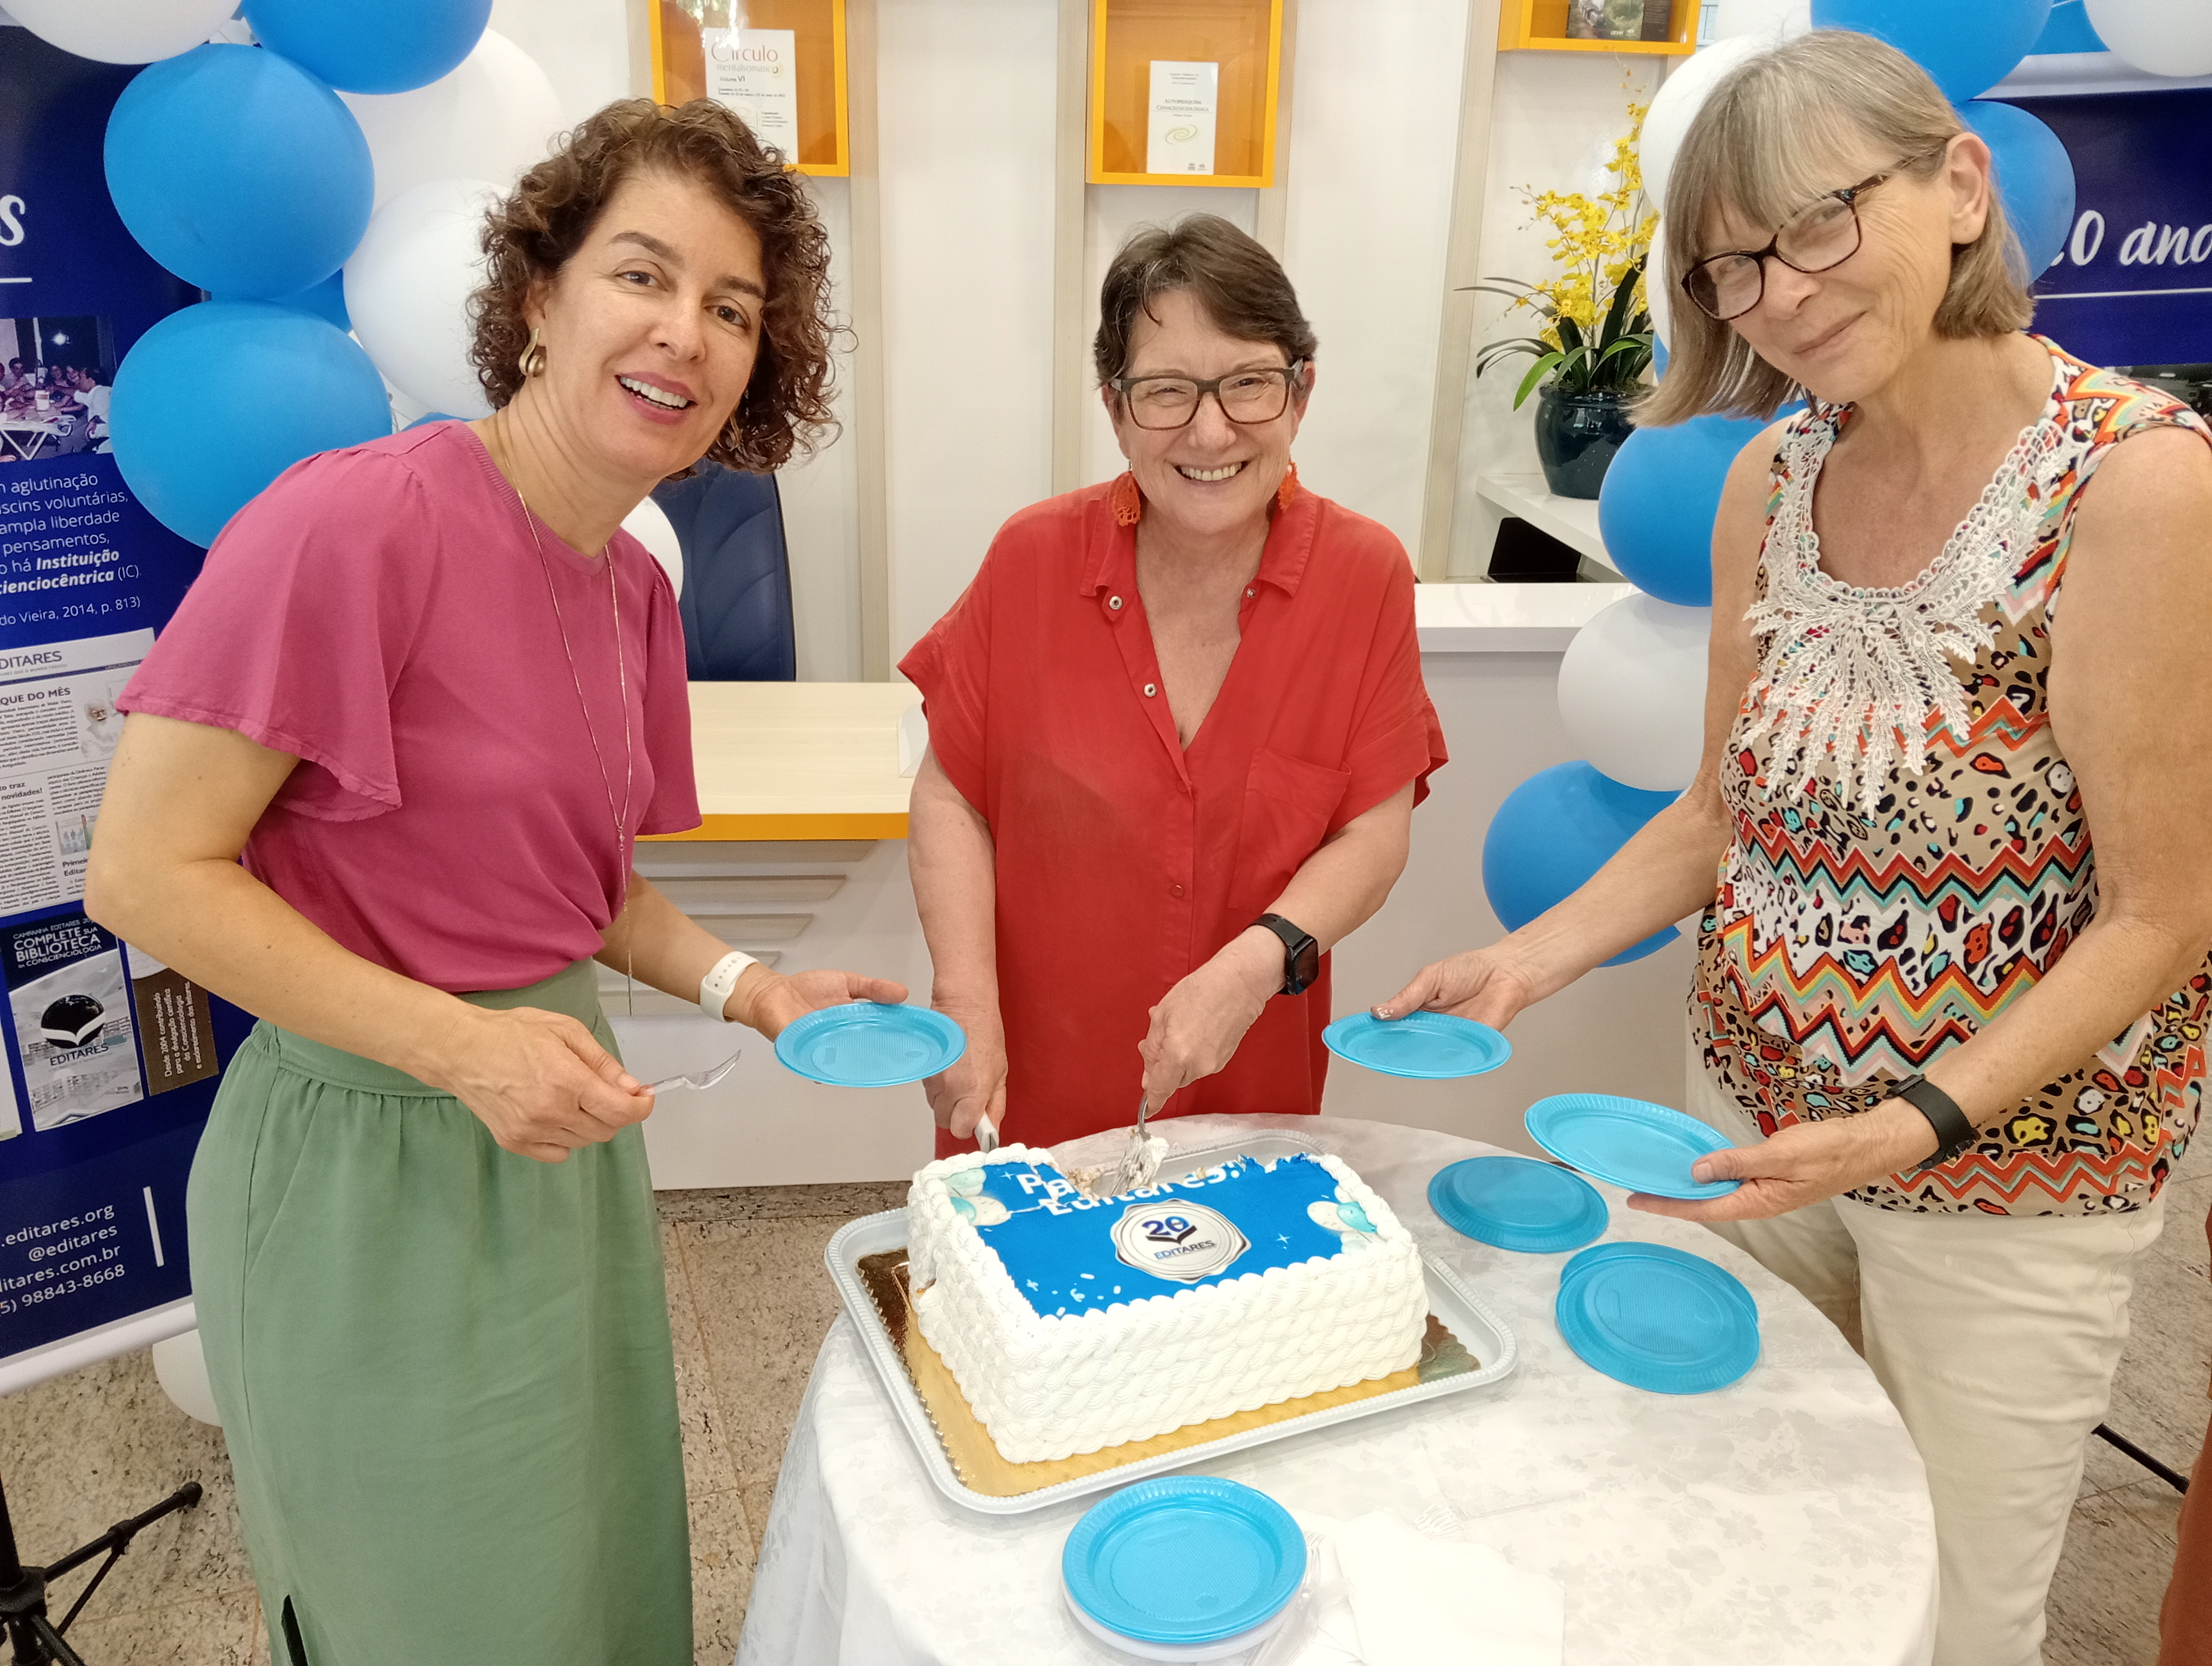
\includegraphics[width=9cm, height=9cm]{articles/resumo/fotos/materia1/IMG20241023143149.jpg}
        
%    \end{multicols}
\end{document}
